\documentclass[10pt]{article}
\usepackage{icmlko}

\icmlmeta{IP 파운데이션 월드모델}{31}{유의한 것과 쓸모 있는 것}{절대량의 성패는 순위 상관이 정한다 --- 게임은 p$<$0.001로 유의한데 r=0.344라 진다}

\begin{document}

\twocolumn[
\icmlheader

\begin{abstract}
게임은 순위 전이가 유의한데(팝업 $\to$ 게임 p=0.0003, 아이돌 $\to$ 게임 p=0.0013)
절대량 단계에서는 상수에 진다(승률 19\%). 노트 30이 그 모순을 미결로 남겼다.
분해했다. \textbf{순위 상관이 전부를 설명한다} --- 아이돌 r=$+$0.681이 가능한
개선폭의 35.7\%를 달성하고, 팝업 r=$+$0.445가 1.3\%, 게임 r=$+$0.344가
$-$9.1\%다. 순서가 정확히 상관 순서다. 그리고 \textbf{눈금에는 문제가 없다} ---
순위를 완전히 안다고 가정하면 배수 오차가 팝업 1.12배, 게임 1.22배, 아이돌
1.76배까지 내려간다. 중심과 중앙절대편차 두 모수로 잡는 눈금은 충분하고,
병목은 순위 품질이다. 여기서 이 프로젝트의 통계 관행에 대한 교훈이 나온다 ---
\textbf{순열 검정이 통과했다고 쓸 수 있는 것이 아니다.} 게임은 n=482라 r=0.344도
p$<$0.001이 된다. 유의성은 ``전이가 없다''를 기각할 뿐 ``예측에 쓸 만하다''를
말하지 않는다. 실무 문턱을 r$\geq$0.5로 잡는다 --- 그 아래에서는 절대량 단계로
넘어가지 않는다.
\end{abstract}
]

\section{모순을 분해한다}

노트 30까지 두 사실이 나란히 있었다.

\begin{itemize}[leftmargin=1.1em,itemsep=0.15em]
\item 게임을 대상으로 한 순위 전이가 유의하다 --- 팝업 $\to$ 게임 p=0.0003,
      아이돌 $\to$ 게임 p=0.0013.
\item 그런데 절대량 단계에서 상수에 진다 --- k=50에서 승률 19\%.
\end{itemize}

절대량은 순위에 눈금을 얹는 것이므로, 순위가 되는데 절대량이 안 된다면 눈금이
문제이거나 순위의 \emph{질}이 문제다. 갈랐다.

\begin{table}[t]
\centering\tsize
\caption{도메인별 진단. 배수 오차는 전량 눈금 기준.}
\begin{tabular}{lrrrr}
\toprule
도메인 & 순위 상관 & 상수 & 현재 & 완전 순위 \\
\midrule
아이돌 & $+$0.681 & 4.41배 & 3.47배 & 1.76배 \\
팝업 & $+$0.445 & 2.66배 & 2.64배 & 1.12배 \\
게임 & $+$0.344 & 3.53배 & 3.74배 & 1.22배 \\
\bottomrule
\end{tabular}
\end{table}

\begin{figure}[t]
\centering
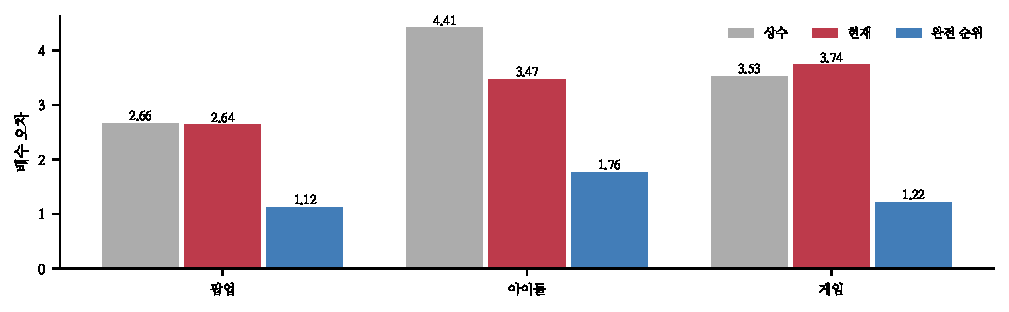
\includegraphics[width=\textwidth]{figs/ceil.pdf}
\caption{상수, 현재, 완전 순위의 배수 오차. 완전 순위와 현재의 간격이 크다.}
\end{figure}

\section{눈금은 문제가 아니다}

순위를 완전히 안다고 가정하면 --- 즉 예측 대신 실제 잔차 순위를 넣으면 --- 배수
오차가 팝업 1.12배, 게임 1.22배, 아이돌 1.76배가 된다.

중심과 중앙절대편차 두 모수로 잡는 눈금이 그 정도까지 간다는 뜻이다. 상수 대비
58\%에서 66\%를 줄인다. \textbf{눈금은 충분하다.}

\claimx{절대량 파이프라인의 눈금(중심 $+$ 중앙절대편차)은 병목이 아니다. 순위를
완전히 알면 배수 오차가 1.1--1.8배까지 내려간다.}{눈금을 더 정교하게 잡아
(분위수 사상 등) 완전 순위 조건에서 1.1배 아래로 내려가면 눈금에도 여지가 있는
것이다.}

\section{순위 상관이 전부를 설명한다}

가능한 개선폭 중 실제로 달성한 비율을 보면 순서가 명확하다.

\begin{figure}[t]
\centering

\includegraphics[width=\columnwidth]{figs/rank.pdf}
\caption{순위 상관과 달성률. 세 점이 직선 위에 있다.}
\end{figure}

\begin{table}[t]
\centering\tsize
\caption{순위 품질과 달성률.}
\begin{tabular}{lrrr}
\toprule
도메인 & 순위 상관 & 개선 여지 & 달성률 \\
\midrule
아이돌 & $+$0.681 & 60.1\% & \textbf{35.7\%} \\
팝업 & $+$0.445 & 58.0\% & 1.3\% \\
게임 & $+$0.344 & 65.5\% & \textbf{$-$9.1\%} \\
\bottomrule
\end{tabular}
\end{table}

개선 여지는 셋 다 58\%에서 66\%로 비슷한데 달성률이 갈린다. 그리고 그 순서가
정확히 순위 상관의 순서다.

게임은 달성률이 음수다 --- 순위 예측을 얹으면 상수보다 나빠진다. r=0.344짜리
순위에 폭을 곱하면 맞는 만큼 틀리는 것이 더 크다.

\claimx{절대량 단계의 성패는 순위 상관이 정한다. 눈금 여지는 도메인마다 비슷하고,
달성률만 상관 순서를 따른다.}{네 번째 도메인에서 상관은 높은데 달성률이 낮거나
그 반대가 나오면 다른 요인이 있다.}

\section{유의성은 쓸모를 보장하지 않는다}

여기서 이 프로젝트의 통계 관행에 대한 교훈이 나온다.

\begin{figure}[t]
\centering

\includegraphics[width=\columnwidth]{figs/sig.pdf}
\caption{순위 상관과 순열 p. 유의성은 셋 다 높은데 상관은 두 배 차이 난다.}
\end{figure}

게임의 순위 전이는 p=0.0003으로 매우 유의하다. 그런데 상관이 0.344다. n=482이므로
그 정도 상관도 우연으로 나오기 어렵다 --- 유의성은 표본 크기에 딸린다.

\textbf{순열 검정이 기각하는 것은 ``전이가 전혀 없다''이지 ``예측에 쓸 만하다''가
아니다.} 이 프로젝트는 스물여섯 편 동안 순열 p로 방향을 판정해 왔고, 그 판정 자체는
옳았다. 다만 그것을 ``쓸 수 있다''로 읽으면 안 된다.

\begin{quote}\fontsize{9.5}{11.5}\selectfont
\textbf{실무 문턱을 r$\geq$0.5로 잡는다.} 순위 상관이 그 아래면 전이가 유의해도
절대량 단계로 넘어가지 않는다. 현재 아이돌만 넘고(0.681) 팝업은 경계(0.445),
게임은 못 넘는다(0.344).
\end{quote}

\claimx{순열 유의성과 실용 가능성은 다른 기준이다. 표본이 크면 낮은 상관도
유의해지므로, 전이 판정 뒤에 순위 상관을 따로 봐야 한다.}{상관이 0.5 아래인데
절대량이 상수를 안정적으로 이기는 사례가 나오면 문턱을 낮춰야 한다.}

\section{부수 --- 진단 스크립트에서 낸 실수}

이 분석을 처음 돌렸을 때 팝업의 배수 오차가 무한대, 아이돌이 NaN으로 나왔다.
원인은 \texttt{raw\_labels}의 반환 순서를 잘못 받은 것이었다 --- 세 번째 값이
추세가 아니라 관측 시점인데 추세로 썼다. 파이프라인 본체는 올바르게 쓰고 있었고
임시 진단 스크립트만 틀렸다.

기록해 두는 이유는 \emph{이상한 수치가 나왔을 때의 순서}다. 무한대와 NaN을 보고
데이터나 방법을 의심하기 전에 배열 정렬부터 확인했더니 5분이면 끝났다.
노트 25에서 배운 것 --- ``요약 통계가 이상할 때는 도메인을 의심하기 전에 배선을
의심한다'' --- 이 코드 수준에서도 같다.

\section{그래서 무엇을 해야 하나}

순위 상관을 올리는 것이 유일한 지렛대다. 두 경로가 있다.

\paragraph{축을 늘린다}
노트 27이 보였듯 관측 축이 늘면 대상으로서 쉬워진다. 게임은 공유 축 둘뿐이고
입장 허들은 여러 노트째 미해결이다.

\paragraph{출처를 늘린다}
현재 순위 예측은 다른 두 도메인 예측의 단순 평균이다. 도메인이 늘면 평균의
분산이 줄어 상관이 오를 수 있다. 노트 22는 표본 확대의 수익이 200건에서 끝난다고
했지만 \emph{도메인} 확대는 다른 축이다.

\section{한계}

\begin{itemize}[leftmargin=1.1em,itemsep=0.15em]
\item 세 점으로 상관과 달성률의 관계를 그렸다. 직선으로 보이지만 점이 셋이다.
\item ``완전 순위''는 대상 라벨을 그대로 쓰므로 도달 불가능한 기준이다.
      실현 가능한 상한은 그보다 낮다.
\item r$\geq$0.5 문턱은 세 도메인의 배치에서 눈으로 그은 선이다. 이론적 근거가 없다.
\item 순위 상관은 전량 라벨로 쟀다. 실전에서는 k건으로 추정해야 하는데 그 추정의
      분산을 보지 않았다.
\end{itemize}

\section{다음}

\begin{enumerate}[leftmargin=1.3em,itemsep=0.15em]
\item k건으로 순위 상관을 추정하는 방법 --- 문턱 판정을 실전에서 쓰려면 필요하다.
\item 입장 허들의 게임 측정 경로.
\item 네 번째 도메인 --- 출처 확대로 순위 상관이 오르는지.
\item 눈금을 분위수 사상으로 바꿔 완전 순위 조건의 하한 재측정.
\end{enumerate}

\vspace{0.6em}
\hrule height 0.3pt
\vspace{0.5em}
{\footnotesize
\textbf{참고문헌}\\[0.3em]
Cohen, J. (1988). \emph{Statistical Power Analysis for the Behavioral Sciences},
2nd ed. Lawrence Erlbaum.\\[0.15em]
Wasserstein, R. L., Lazar, N. A. (2016). The ASA statement on p-values.
\emph{The American Statistician}, 70(2), 129--133.\\[0.15em]
Good, P. (2005). \emph{Permutation, Parametric, and Bootstrap Tests of Hypotheses},
3rd ed. Springer.\\[0.15em]
Ben-David, S. et al. (2010). A theory of learning from different domains.
\emph{Machine Learning}, 79(1--2), 151--175.
}

\end{document}
